\documentclass{article}

\usepackage{graphicx}


\begin{document}

\section*{1.8}

\subsection*{a}

Consider the graph

\begin{figure}[h]
	\centering
	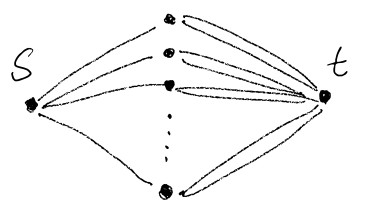
\includegraphics{graph1.jpg}
\end{figure}

Removing any edge on the left side will increase the min cut. 
Initially the left-side edges make up $\frac{1}{3}$ of the total amount of edges.
At every stage if the algorithm has not contracted any wrong edge, the probability of contracting a wrong edge is than at least $\frac{1}{3}$. Thus we see that the probability of obtaining the min-cut is at most

$$ \left(\frac{2}{3}\right)^{n-1} $$

Where $n$ is the total number of edges. (This is exponentially decreasing in $n$).


\end{document}

